% Dokumentenkopf ---------------------------------------------------------------
%   Diese Vorlage basiert auf "scrreprt" aus dem koma-script.
% ------------------------------------------------------------------------------
\documentclass[
	ngerman,
    11pt, % Schriftgr??e
    DIV10, % Seitengroesse (siehe Koma Skript Dokumentation !)
    ngerman, % f?r Umlaute, Silbentrennung etc.
    a4paper, % Papierformat
    oneside, % einseitiges Dokument
    titlepage, % es wird eine Titelseite verwendet
    parskip=half, % Abstand zwischen Abs?tzen (halbe Zeile)
    headings=normal, % Gr??e der ?berschriften verkleinern
%	chapterprefix=true, % Ausgabe Kapitel + Nummer
    listof=totoc, % Verzeichnisse im Inhaltsverzeichnis auff?hren
	bibliography=totoc, % Literaturverzeichnis im Inhaltsverzeichnis auff?hren
    index=totoc, % Index im Inhaltsverzeichnis auff?hren
    captions=tableheading, % Beschriftung von Tabellen unterhalb ausgeben
    final, % Status des Dokuments (final/draft)
	pointlessnumbers % keine Nummern hinter Kapitelnummern
%	numbers=noenddot
	abstracton % Erzeugen einer Zusammenfassung
]{scrartcl}


% Meta-Informationen -----------------------------------------------------------
%   Informationen ?ber das Dokument, wie z.B. Titel, Autor, Matrikelnr. etc
%   werden in der Datei Meta.tex definiert und k?nnen danach global
%   verwendet werden.
% ------------------------------------------------------------------------------
% Meta-Informationen -----------------------------------------------------------
%   Definition von globalen Parametern, die im gesamten Dokument verwendet
%   werden k�nnen (z.B auf dem Deckblatt etc.).
%
%   ACHTUNG: Wenn die Texte Umlaute oder ein Esszet enthalten, muss der folgende
%            Befehl bereits an dieser Stelle aktiviert werden:
%            \usepackage[latin1]{inputenc}
% ------------------------------------------------------------------------------

\newcommand{\titel}{Praktikum Embedded- und Echtzeitbetriebssysteme}
\newcommand{\titeleng}{xy}
\newcommand{\untertitel}{}
\newcommand{\art}{Studienarbeit}
\newcommand{\fachgebiet}{Fakult�t f�r Informatik und Mathematik}
\newcommand{\autor}{Maximilian Hempe und Roland Wilhelm}
%\newcommand{\autor2}{Maximilian Hempe}
\newcommand{\studienbereich}{Embedded Computing}
\newcommand{\matrikelnr}{12 34 56}
\newcommand{\erstgutachter}{xy}
\newcommand{\zweitgutachter}{xyz}
\newcommand{\jahr}{2012}
\newcommand{\ort}{Hochschule M�nchen}
%\newcommand{\logo}{}


% ben?tigte Packages -----------------------------------------------------------
%   LaTeX-Packages, die ben?tigt werden, sind in die Datei Packages.tex
%   "ausgelagert", um diese Vorlage m?glichst ?bersichtlich zu halten.
% ------------------------------------------------------------------------------
% Anpassung des Seitenlayouts --------------------------------------------------
%   siehe Seitenstil.tex
% ------------------------------------------------------------------------------
\usepackage[
    automark, % Kapitelangaben in Kopfzeile automatisch erstellen
    headsepline, % Trennlinie unter Kopfzeile
    ilines % Trennlinie linksb�ndig ausrichten
]{scrpage2}

% Anpassung an Landessprache ---------------------------------------------------
\usepackage[ngerman]{babel}

% Umlaute ----------------------------------------------------------------------
%   Umlaute/Sonderzeichen wie ���� direkt im Quelltext verwenden (CodePage).
%   Erlaubt automatische Trennung von Worten mit Umlauten.
% ------------------------------------------------------------------------------
\usepackage[latin1]{inputenc}
\usepackage[T1]{fontenc}
\usepackage{textcomp} % Euro-Zeichen etc.



% Schrift ----------------------------------------------------------------------
\usepackage{lmodern} % bessere Fonts
\usepackage{relsize} % Schriftgr��e relativ festlegen

% Grafiken ---------------------------------------------------------------------
% Einbinden von JPG-Grafiken erm�glichen
\usepackage[dvips,final]{graphicx}
% hier liegen die Bilder des Dokuments
\graphicspath{{Bilder/}}

% Befehle aus AMSTeX f�r mathematische Symbole z.B. \boldsymbol \mathbb --------
\usepackage{amsmath,amsfonts}

% f�r Index-Ausgabe mit \printindex --------------------------------------------
\usepackage{makeidx}

% Einfache Definition der Zeilenabst�nde und Seitenr�nder etc. -----------------
\usepackage{setspace}
\usepackage{geometry}

% Einfaches Packet um ganze Bl�cke als Kommentar zu kennzeichnen z.b. \begin{comment} ... \end{comment}
\usepackage{comment}


% erm�glicht das einbinden von pdf Dateien oder nur bestimmte Seiten
\usepackage{pdfpages}

% Symbolverzeichnis ------------------------------------------------------------
%   Symbolverzeichnisse bequem erstellen. Beruht auf MakeIndex:
%     makeindex.exe %Name%.nlo -s nomencl.ist -o %Name%.nls
%   erzeugt dann das Verzeichnis. Dieser Befehl kann z.B. im TeXnicCenter
%   als Postprozessor eingetragen werden, damit er nicht st�ndig manuell
%   ausgef�hrt werden muss.
%   Die Definitionen sind ausgegliedert in die Datei "Glossar.tex".
% ------------------------------------------------------------------------------
%\usepackage[intoc]{nomencl}
%\let\abbrev\nomenclature
%\renewcommand{\nomname}{Abk�rzungsverzeichnis}
%\setlength{\nomlabelwidth}{.25\hsize}
%\renewcommand{\nomlabel}[1]{#1 \dotfill}
%\setlength{\nomitemsep}{-\parsep}

% Abk�rzungsverzeichnis, Abk�rzungen werden nur angezeigt wenn diese im Text auch benutzt werden
\usepackage[printonlyused]{acronym}


% zum Umflie�en von Bildern ----------------------------------------------------
\usepackage{floatflt}


% zum Einbinden von Programmcode -----------------------------------------------
\usepackage{listings}
\usepackage{xcolor} 
\definecolor{hellgelb}{rgb}{1,1,0.9}
\definecolor{colKeys}{rgb}{0,0,1}
\definecolor{colIdentifier}{rgb}{0,0,0}
\definecolor{colComments}{rgb}{1,0,0}
\definecolor{colString}{rgb}{0,0.5,0}
\lstset{
    float=hbp,
    basicstyle=\ttfamily\color{black}\small\smaller,
    identifierstyle=\color{colIdentifier},
    keywordstyle=\color{colKeys},
    stringstyle=\color{colString},
    commentstyle=\color{colComments},
    columns=flexible,
    tabsize=2,
    frame=single,
    extendedchars=true,
    showspaces=false,
    showstringspaces=false,
    numbers=left,
    numberstyle=\tiny,
    breaklines=true,
    backgroundcolor=\color{hellgelb},
    breakautoindent=true
}

% URL verlinken, lange URLs umbrechen etc. -------------------------------------
\usepackage{url}

% wichtig f�r korrekte Zitierweise ---------------------------------------------
\usepackage[square,numbers]{natbib}

% PDF-Optionen -----------------------------------------------------------------
\usepackage[
    bookmarks,
    bookmarksopen=true,
    colorlinks=true,
% diese Farbdefinitionen zeichnen Links im PDF farblich aus
    linkcolor=black, % einfache interne Verkn�pfungen, default:red
    anchorcolor=black,% Ankertext, default:black
    citecolor=black, % Verweise auf Literaturverzeichniseintr�ge im Text, default:blue
    filecolor=black, % Verkn�pfungen, die lokale Dateien �ffnen, default:magenta
    menucolor=black, % Acrobat-Men�punkte, default:red
    urlcolor=black, 
% diese Farbdefinitionen sollten f�r den Druck verwendet werden (alles schwarz)
    %linkcolor=black, % einfache interne Verkn�pfungen
    %anchorcolor=black, % Ankertext
    %citecolor=black, % Verweise auf Literaturverzeichniseintr�ge im Text
    %filecolor=black, % Verkn�pfungen, die lokale Dateien �ffnen
    %menucolor=black, % Acrobat-Men�punkte
    %urlcolor=black, 
    backref,
    plainpages=false, % zur korrekten Erstellung der Bookmarks
    pdfpagelabels, % zur korrekten Erstellung der Bookmarks
    hypertexnames=false, % zur korrekten Erstellung der Bookmarks
    linktocpage % Seitenzahlen anstatt Text im Inhaltsverzeichnis verlinken
]{hyperref}
% Befehle, die Umlaute ausgeben, f�hren zu Fehlern, wenn sie hyperref als Optionen �bergeben werden
\hypersetup{
    pdftitle={\titel \untertitel},
    pdfauthor={\autor},
    pdfcreator={\autor},
    pdfsubject={\titel \untertitel},
    pdfkeywords={\titel \untertitel},
}



% fortlaufendes Durchnummerieren der Fu�noten ----------------------------------
\usepackage{chngcntr}

% f�r lange Tabellen -----------------------------------------------------------
\usepackage{longtable}
\usepackage{array}
\usepackage{ragged2e}
\usepackage{lscape}

% Spaltendefinition rechtsb�ndig mit definierter Breite ------------------------
\newcolumntype{w}[1]{>{\raggedleft\hspace{0pt}}p{#1}}

% Formatierung von Listen �ndern -----------------------------------------------
\usepackage{paralist}

% bei der Definition eigener Befehle ben�tigt
\usepackage{ifthen}

% definiert u.a. die Befehle \todo und \listoftodos
\usepackage{todonotes}

% sorgt daf�r, dass Leerzeichen hinter parameterlosen Makros nicht als Makroendezeichen interpretiert werden
\usepackage{xspace}


% Erstellung eines Index und Abk?rzungsverzeichnisses aktivieren ---------------
\makeindex
%\makenomenclature

% Kopf- und Fu?zeilen, Seitenr?nder etc. ---------------------------------------
% Zeilenabstand 1,5 Zeilen -----------------------------------------------------
\onehalfspacing

% Seitenr�nder -----------------------------------------------------------------
\setlength{\topskip}{\ht\strutbox} % behebt Warnung von geometry
\geometry{paper=a4paper,left=35mm,right=35mm,top=30mm}

% Kopf- und Fu�zeilen ----------------------------------------------------------
\pagestyle{scrheadings}
% Kopf- und Fu�zeile auch auf Kapitelanfangsseiten
%\renewcommand*{\chapterpagestyle}{scrheadings} 
% Schriftform der Kopfzeile
\renewcommand{\headfont}{\normalfont}

% Kopfzeile
\ihead{\textit{\headmark}}
\chead{}
\ohead{\pagemark}
\setlength{\headheight}{21mm} % H�he der Kopfzeile
\setheadsepline[text]{0.4pt} % Trennlinie unter Kopfzeile

%\ihead{\large{\textsc{\titel}}\\ \small{\untertitel} \\[2ex] \textit{\headmark}}
%\ohead{\includegraphics[scale=0.15]{\logo}}
% Kopfzeile �ber den Text hinaus verbreitern
%\setheadwidth[0pt]{textwithmarginpar} 


% Fu�zeile
\ifoot{}
\cfoot{}
\ofoot{}

% sonstige typographische Einstellungen ----------------------------------------

% erzeugt ein wenig mehr Platz hinter einem Punkt
\frenchspacing 

% Schusterjungen und Hurenkinder vermeiden
\clubpenalty = 10000
\widowpenalty = 10000 
\displaywidowpenalty = 10000

% Quellcode-Ausgabe formatieren
\lstset{numbers=left, numberstyle=\tiny, numbersep=5pt, breaklines=true}
\lstset{emph={square}, emphstyle=\color{red}, emph={[2]root,base}, emphstyle={[2]\color{blue}}}

% Fu�noten fortlaufend durchnummerieren
\counterwithout{footnote}{section}


% eigene Definitionen f?r Silbentrennung
% Trennvorschl�ge im Text werden mit \" angegeben
% untrennbare W�rter und Ausnahmen von der normalen Trennung k�nnen in dieser
% Datei mittels \hyphenation definiert werden

% eigene LaTeX-Befehle
% Eigene Befehle und typographische Auszeichnungen f�r diese

% einfaches Wechseln der Schrift, z.B.: \changefont{cmss}{sbc}{n}
\newcommand{\changefont}[3]{\fontfamily{#1} \fontseries{#2} \fontshape{#3} \selectfont}

% Abk�rzungen mit korrektem Leerraum 
\newcommand{\ua}{\mbox{u.\,a.\ }}
\newcommand{\zb}{\mbox{z.\,B.\ }}
\newcommand{\dahe}{\mbox{d.\,h.\ }}
\newcommand{\vgl}{Vgl.\ }
\newcommand{\bzw}{bzw.\ }
\newcommand{\evtl}{evtl.\ }
\newcommand{\uvm}{\mbox{u.\,v.\,m.\ }}
%\newcommand{\dh}{\mbox{d.\,h.\ }}

\newcommand{\Abbildung}[1]{Abbildung~\ref{abb:#1}}

\newcommand{\bs}{$\backslash$}

% erzeugt ein Listenelement mit fetter �berschrift 
\newcommand{\itemd}[2]{\item{\textbf{#1}}\\{#2}}

% einige Befehle zum Zitieren --------------------------------------------------
\newcommand{\Zitat}[2][\empty]{\ifthenelse{\equal{#1}{\empty}}{\citep{#2}}{\citep[#1]{#2}}}

% zum Ausgeben von Autoren
\newcommand{\AutorName}[1]{\textsc{#1}}
\newcommand{\Autor}[1]{\AutorName{\citeauthor{#1}}}

% verschiedene Befehle um W�rter semantisch auszuzeichnen ----------------------
\newcommand{\NeuerBegriff}[1]{\textbf{#1}}
\newcommand{\Fachbegriff}[1]{\textit{#1}}

\newcommand{\Eingabe}[1]{\texttt{#1}}
\newcommand{\Code}[1]{\texttt{#1}}
\newcommand{\Datei}[1]{\texttt{#1}}
\newcommand{\Klasse}[1]{\texttt{#1}}
\newcommand{\Interface}[1]{\texttt{#1}}
\newcommand{\Komponente}[1]{\mbox{\glqq {#1}\grqq}}
\newcommand{\Anf}[1]{\mbox{\glqq {#1}\grqq}}


\newcommand{\Datentyp}[1]{\textsf{#1}}
\newcommand{\XMLElement}[1]{\textsf{#1}}
\newcommand{\Webservice}[1]{\textsf{#1}}


% Das eigentliche Dokument -----------------------------------------------------
%   Der eigentliche Inhalt des Dokuments beginnt hier. Die einzelnen Seiten
%   und Kapitel werden in eigene Dateien ausgelagert und hier nur inkludiert.
% ------------------------------------------------------------------------------
\begin{document}

% auch subsubsection nummerieren
\setcounter{secnumdepth}{3}
\setcounter{tocdepth}{3}

% Deckblatt und Abstract ohne Seitenzahl
\ohead{}
\begin{titlepage}
	\begin{center}		
		\vspace*{1cm} % * forces the space, else the space will not be shown
		\vspace*{1cm}
		
		\begin{center}
			
\includegraphics[width=0.90\textwidth]{Bilder/hm.png}
		\end{center}
		\vspace{1.0cm}
		{\Huge Computational Geometry\\}
		\vspace{1.0cm}
		{\Large Ausarbeitung f�r das Praktikum}\\
		\vspace{1cm}
		{\Large Studienarbeit von}\\
		\vspace{0.1cm}
		{\Large Maximilian Hempe}\\
		{\Large Roland Wilhelm}\\
		
		
		\vspace*{4.0cm}
		
		{\normalsize Dozent: Dr. Fischer} \\
		{\normalsize Hochschule M�nchen} \\
		{\normalsize Master Informatik} \\	
		{\normalsize \today}		
		
		\vspace{1.5cm}		
	
	  \vspace{2cm}		
	\end{center} 
\end{titlepage}
%\includegraphics[width=1.00\textwidth]{thema.pdf}
%\includegraphics[width=1.00\textwidth]{erklaerung.pdf}
%\includepdf{thema.pdf} 
% Selbst?ndigkeitserkl?rung
\ohead{\pagemark}

% Seitennummerierung -----------------------------------------------------------
%   Vor dem Hauptteil werden die Seiten in gro?en r?mischen Ziffern 
%   nummeriert.
% ------------------------------------------------------------------------------
%\pagenumbering{Roman}
%\include{Inhalt/Abstract}

% Inhaltverzeichnis im PDF anzeigen aber nicht im Inhaltverzeichnis selbst
%\clearpage %%% ggf. \cleardoublepage
%\phantomsection
\clearpage
\pdfbookmark{\contentsname}{toc}
\tableofcontents %die Tilden zum Einrücken im Bookmark

%\tableofcontents % Inhaltsverzeichnis
\clearpage
\listoffigures % Abbildungsverzeichnis
%\clearpage
%\listoftables % Tabellenverzeichnis
\clearpage
\renewcommand{\lstlistlistingname}{Listingsverzeichnis}
\lstlistoflistings % Listings-Verzeichnis


% Abk?rzungsverzeichnis --------------------------------------------------------
%\addsec{Abk�rzungsverzeichnis} %�berschrift im Inhaltsverueichnis auflisten aber ohne Nummerierung
\begin{acronym} %[Abk.] l�ngste form angeben zum ausrichten
%\ac{Abk.}         % f�gt die Abk�rzung ein, au�er beim ersten Aufruf, hier wird die Erkl�rung mit angef�gt
%\acs{Abk.}        % f�gt die Abk�rzung ein
%\acf{Abk.}        % f�gt die Abk�rzung UND die Erkl�rung ein
%\acl{Abk.}        % f�gt nur die Erkl�rung ein
%\acro{3GPP}{3rd Generation Partnership Project}	% Hinzuf�gen einer neuen Abk�rzung


\end{acronym}

%\nomenclature{API}{Application Programming Interface}
\nomenclature{ARIS}{Architektur integrierter Informationssysteme}
\nomenclature{BPR}{Business Process Reengineering}
\nomenclature{eEPK}{erweiterte Ereignisgesteuerte Prozesskette}
\nomenclature{EPK}{Ereignisgesteuerte Prozesskette}
\nomenclature{JMS}{Java Message Service}
\nomenclature{SDK}{Software Development Kit}
\nomenclature{URI}{Uniform Resource Identifier}
\nomenclature{URL}{Uniform Resource Locator}
\nomenclature{URN}{Uniform Resource Name}
\nomenclature{W3C}{World Wide Web Consortium}
\nomenclature{XML}{Extensible Markup Language}
\nomenclature{XPath}{XML Path Language}
\nomenclature{XSL}{Extensible Stylesheet Language}
\nomenclature{XSLT}{XSL Transformations}

% f?r korrekte ?berschrift in der Kopfzeile
%\clearpage\markboth{\nomname}{\nomname} 
%\printnomenclature
%\label{sec:Glossar}


% arabische Seitenzahlen im Hauptteil ------------------------------------------
\clearpage
\pagenumbering{arabic}

% die Inhaltskapitel werden in "Inhalt.tex" inkludiert -------------------------
%\linespread{3.0}
% Hier k�nnen die einzelnen Kapitel inkludiert werden. Sie m�ssen in den 
% entsprechenden .TEX-Dateien vorliegen. Die Dateinamen k�nnen nat�rlich 
% angepasst werden.

\section{Einleitung}
\label{sec:Einleitung}

Diese Studienarbeit beschreibt das Praktikum zur Vorlesung Embedded- und Echtzeitbetriebssysteme. Die Studenten sollen darin
den Umgang mit Betriebssystemen von Embedded Systemen kennenlernen. Die grundlegenden Werkzeuge im Praktikum sind ein BeagleBoard, 
das Echtzeitbetriebssystem QNX und die dazugeh�rige Entwicklungsumgebung QNX Momentics.
Auf dieser Basis werden im Verlauf mehrere Aufgaben erarbeitet. Diese vertiefen die Themen der Vorlesung und gehen auf spezielle 
Sachverhalte intensiver ein. Ziel ist es zyklisch Threads zu starten und mit Hilfe einer selbstentwickelten zeitverschwende Funktion 
das Embedded System auszulasten. Diese Auslastung wird mit Hilfe von Momentics dargestellt und es kann analysiert werden, ob die 
Threads ihre Echtzeitbedingungen einhalten k�nnen. Abschlie�end wird der QNX Kernel noch optimiert, sodass er lediglich die unbedingt
n�tigen Module enth�lt.

\section{Aufgabe 1}
\label{sec:Aufgabe1}
In dieser Aufgabe soll eine Datei mit Liniensegmenten eingelesen werden und die Liniensegmente anschlie{\ss}end auf Schnittpunkte überprüft werden. Ein Liniensegment besitzt im Gegensatz zu einer Geraden einen Start- und einen Endpunkt. Diese Punkte sind je durch X- und Y-Koordinate definiert. Eine Zeile in der einzulesenden Datei enthält pro Zeile die beiden Koordinaten von Beginn und Ende des Segments.

Der Algorithmus sollte zu Beginn möglichst einfach sein, deshalb wird jede Linie mit jeder anderen Linie auf einen Schnittpunkt getestet. Dadurch entsteht eine abstrakte Laufzeit von O\(n²\).

Um den Algorithmus testen zu können gab es drei verschieden gro{\ss}e Files, eine mit 1000 Segmenten, eine mit 10.000 Segmenten und eine mit 100.000 Segmenten. Die Laufzeit verlängert sich bei verzehnfachung der Linien um ca. das 100 Fache.

\subsection{Einlesen der Daten}
\label{subsec:A1_EinlesenDaten}




\subsection{Ablauf des Algorithmus}
\label{subsec:A1_Algorithmus}
Nachdem die Segmente eingelesen sind, wird die Funktion zur Berechnung der sich schneidenden Linien aufgerufen. Darin enthalten ist die Zeitmessung, diese wird direkt am Funktionsbeginn gestartet und vor der Rückgabe beendet. 

Jede Linie muss immer nur ein Mal mit jeder anderen Linie auf mindestens einen gemeinsamen Punkt getestet werden. Deshalb wird der Test in einer verschachtelten Schleife so realisiert, dass die innere Schleife immer nur nachfolgende Linien abfrägt. Doppelte Abfragen, wie Linie 3 mit Linie 4 und Linie 4 mit Linie 3, werden somit verhindert.

\begin{lstlisting}
	for(unsigned int i = 0; i < m_lines.size(); i++) {
		for(unsigned int j = i+1; j < m_lines.size(); j++) {

			if(m_lines[i]->is_intersection(m_lines[j]) == true) {
				m_intersected_lines_nr++;
			}
		}
	}
\end{lstlisting}

Ergibt der Test auf einen Schnittpunkt ein true, wird eine Membervariable um inkrementiert. Der Algorithmus terminiert wenn das Array, das die Segmente beinhaltet, komplett geprüft wurde. Das Ergebnis ist die Anzahl der Schnittpunkte, die durch die Membervariable festgehalten wird.

\subsection{Test auf Schnittpunkte}
Der Test ob es einen Schnittpunkt gibt, muss in diesem Fall in zwei Abschnitte geteilt werden. Im ersten Abschnitt wird geprüft, ob die Punkte der einen Linie auf der selben Seite der anderen Linie liegen. Das wird mit Hilfe einer Funktion geprüft, die testet ob die übergebenen Punkte gegen den Urzeigersinn verlaufen oder nicht.

Liegen Start- und Endpunkt der anderen Linie, aus sicht beider Strecken, je auf verschiedenen Seiten, gibt es einen Schnittpunkt.

\begin{lstlisting}
else if ( (ccw_max(m_start, m_end, a_line->m_start)*ccw_max(m_start, m_end, a_line->m_end)) < 0
		  && ccw_max(a_line->m_start, a_line->m_end, m_start)*ccw_max(a_line->m_start, a_line->m_end, m_end) < 0 ) {

	//->Schnittpunkt!!
	return true;
}
\end{lstlisting}
 
Zuerst werden die beiden Linien auf Kolinierität geprüft, das würde bedeuten, dass ein Dreieck aus drei der vier Punkte keine Fläche aufspannt.
Falls die Linie ein Punkt ist, wird nun vereinfacht geprüft, ob dieser Punkt auf der anderen Strecke liegt. Ist das der Fall, hat man bereits einen Schnittpunkt gefunden, falls nicht gibt es keinen Schnittpunkt.
\begin{lstlisting}
if ( ccw_max(m_start, m_end, a_line->m_start) == 0 && ccw_max(m_start, m_end, a_line->m_end) == 0) {
	if ( m_start == m_end ) {

		//Punkt liegt auf Linie??
		if( ( m_start > a_line->m_start && m_start < a_line->m_end )
			|| (m_start < a_line->m_start && m_start > a_line->m_end)){
			return true;
		}
		else
			return false;
\end{lstlisting}

Ist die Linie regulär, hat sie also einen vom Startpunkt unterschiedlichen Endpunkt, muss ein \"Uberlappungstest durchgeführt werden.

Hierfür wird der Verktor aus Start- und Endpunkt um 90 Grad und -90 Grad gedreht, sodass zwei zusätzliche Punkte über der Linie entstehen. Nun wird getestet ob die Dreiecke aus Startpunkt, neuem Punkt und einem Punkt der anderen Linie bzw. Endpunkt, zweitem neuem Punkt und dem anderen Punkt der anderen Linie in gleicher Richtung verlaufen. Das bedeutet, Start- und'/oder Endpunkt sind nicht beide auf der gleichen Seite der Strecke - also nicht kolinear.
Ist das der Fall, handelt es sich um eine \"Uberlappung.
\begin{lstlisting}
else { //überlappungstest (line <-> line oder line <-> punkt)
			 //p über m_start - drehung um -90°, q über m_end - drehung um 90° des gegengesetzten Vektor
		Point p(m_end.get_y()-m_start.get_y(), m_end.get_x()-m_start.get_x()),
				  q(m_start.get_y()-m_end.get_y(), m_end.get_x()-m_start.get_x());

		//Start-Punkt auf der Linie (inkl Ränder)
		if( ccw_max(m_start, a_line->m_start, p)*ccw_max(m_end,q,a_line->m_start) >= 0 ){
			return true;
		}
		//End-Punkt auf der Linie (inkl Ränder)
		else if(ccw_max(m_start, a_line->m_end, p)*ccw_max(m_end,q,a_line->m_end) >= 0){
			return true;
		}
		else
			return false;
	}
}
\end{lstlisting}

Sind beide Tests negativ, gibt es keinen Schnittpunkt. Es kann also ein sonst generell gültiger Else-Fall erstellt werden, der false zurück liefert.

\label{subsec:A1_Schnittpunkte}



\section{Aufgabe 2}
\label{sec:Aufgabe2}

\section{Aufgabe 3 - Line Sweep}
\label{sec:Aufgabe3}
Der Line Sweep Algorithmus ist ein Versuch die Schnittpunkt suche zu beschleunigen. Die Laufzeit wird nun outputsensitiv, also abh�ngig von der Anzahl der gefundenen Schnittpunkte. Es wird eine fiktive vertikale Linie erzeugt, die sich Punkt f�r Punkt durch die Linien arbeitet. Bei der Art wird zwischen Anfangs-, End- und Schnittpunkt unterschieden, je nach Art des Punktes werden eine andere Aktionen durchgef�hrt. Schnittpunkte k�nnen immer nur zwischen benachbarten Segmenten auftreten. Der Algorithmus terminiert, wenn alls Punkte bzw. Events bearbeitet wurden.

Es gibt beim Line Sweep allerdings einige Funktionseinschr�nkungen, die die Gleichzeitigkeit von Ereignissen betreffen. Diese beherrscht er nur mit sehr aufwendig zu implementierenden Mechanismen. Um die Aufgabe nicht unn�tig komplexer zu gestalten werden diese nicht eingebaut und darauf geachtet folgende Regeln einzuhalten:
\begin{itemize}
\item X-Koordinaten von Schnitt- und Endpunkten sind paarweise verschieden
\item L�nge der Segmente >0
\item nur echte Schnittpunkte
\item keine Linien parallel zur Y-Achse
\item keine Mehrfachschnittpunkte
\item keine �berlappenden Segmente
\end{itemize}



\subsection{Initialisierung}
Die Sweep Line besteht aus mehreren Queues, die den aktuellen und zuk�nftigen Zustand verwalten. Die erste Queue ist die Eventqueue, hier werden die Punkte abgelegt und mit der Information versehen, auch welcher Linie sie liegen. Bei Schnittpunkten werden die beiden Linien vermerkt, die sich dort schneiden.
\begin{lstlisting}[captionpos=b, caption={Attribute der Klasse Event}, label=A3:Eventpriv]
class Event {
private:
	MyEventtype m_type;
	Point m_punkt;
	Line* m_seg;
	Line* m_seg2; //falls schnittpunkt
...
\end{lstlisting}

In der zweiten Liste werden die Segmente verwaltet, die sich aktuell mit der Seep Line schneiden. An einem Startpunkt wird die damit verbundene Linie an der richtigen Stelle in diese Queue eingef�gt und auf Schnittpunkte mit ihren Nachbarn �berpr�ft. Erreicht die Sweep Line einen Endpunkt, wird die entsprechende Linie entfernt und die neuen Nachbarn auf einen Schnittpunkt getestet. Wird ein Schnittpunkt behandelt, m�ssen die beiden Segmente auf der dieser Schnittpunkt liegt die Positionen tauschen. Gefundene Schnittpunkte werden in die Output Liste und als neues Event in die Eventqueue eingef�gt. Hier ist besonders darauf zu achten, dass die Schnittpunkte an der richtigen Position einsortiert werden.
\begin{lstlisting}[captionpos=b, caption={Attribute der Klasse Sweep}, label=A3:Sweeppriv]
class Sweep {
private:
	list<Event> eventqueue;
	list<Line> segmentqueue;
	Event *ereignis;
	list<Event> output;
...
\end{lstlisting}

Um die Eventqueue zu initialisieren wurde eine neue Funktion in die Klasse LineFile eingef�gt. Diese f�gt alls Punkte ein und definiert ob es sich um einen Start- oder Endpunkt handelt. Anschlie�end wird die Liste durch eine in der STL enthaltende Funktion nach der X-Koordinate sortiert.
\begin{lstlisting}[captionpos=b, caption={Initialisierung der Sweep Line}, label=A3:Sweepinit]
void LineFile::sweepiniteventqueue(){
	for(unsigned int i = 0; i < m_lines.size(); i++) {
		m_sweep.addevent(m_lines[i]->getstart(),m_lines[i]);
		m_sweep.addevent(m_lines[i]->getend(), m_lines[i]);
	}

}
...
void Sweep::addevent(Point* a_point, Line* a_line){
	//a_point ist startpunkt
	if ( a_point == a_line->getstart() ){
		eventqueue.push_front( Event(a_point, a_line, STARTPUNKT) );
	}
	//a_point ist endpunkt
	else {
		eventqueue.push_front( Event(a_point, a_line, ENDPUNKT) );
	}
	print_eventqueue();
}
\end{lstlisting}



\subsection{Behandlung von Events}
Da die Eventqueue immer nach aufsteigenden X-Koordinaten sortiert sein muss, kann der aktuelle X-Wert der Sweep Line durch die X-Koordinate des ersten Elements in der Eventqueue bestimmt werden. Wird die Sweep gestartet, w�hlt sie das erste Event aus der Queue und f�hrt je nach Art des Punktes die entsprechende Aktion aus. Anschlie�end wird das Event aus der Queue entfernt und wieder das erste ausgew�hlt. Dieser Vorgang wir solange wiederholt, bis keine Events mehr in der Eventqueue enthalten sind. Dann k�nnen die Schnittpunkte aus der Outputqueue ausgelesen werden. Da der Vorgang des Ausw�hlens und L�schen von Events bei allen Punkten gleich ist, wird dieser im Folgenden nicht weiter erw�hnt.
\begin{lstlisting}[captionpos=b, caption={Schleife der Sweep Line}, label=A3:Sweeprun]
void Sweep::calcinters(){
bool test = false;
list<Event>::iterator neweve;

	eventqueue.sort();
	while( (test = eventqueue.empty()) == false) {
		neweve = eventqueue.begin();
		ereignis = &(*neweve);

		switch(ereignis->gettype()){
			case STARTPUNKT:
				leftendpoint( );
				break;

			case ENDPUNKT:
				rightendpoint( );
				break;

			case INTERSECTION:
				treatintersection( );
				break;

			default:
				exit(1);
				break;
		}
		delevent(ereignis);
	}
}
\end{lstlisting}


\subsubsection{Startpunkte}
Wie schon kurz beschrieben, wird bei der Behandlung eines Startpunktes das neue Segment in die Segmentqueue eingef�gt. Es ist wichtig, dass es an der richtigen Stelle eingef�gt wird, da nur zwischen Nachbarn ein Schnittpunkt liegen kann. Ist die Nachbarschaft nicht korrekt sortiert, kommt es zu schwer nachvollziehbaren Fehlern.
\begin{lstlisting}[captionpos=b, caption={Einf�gen von Segmenten in die Sweep Line}, label=A3:addseg]
Line* Sweep::addseg(Line* a_seg) {
	list<Line>::iterator newseg;

	if ( segmentqueue.empty() ) {
		segmentqueue.push_front(*a_seg);
		return a_seg;
	}
	else {
		for ( newseg = segmentqueue.begin(); newseg != segmentqueue.end(); ++newseg ) {
			if ( newseg->get_yvalue(getxposition()) > a_seg->get_yvalue(getxposition()) ) {
				segmentqueue.insert (newseg, *a_seg);
				return a_seg;
			}
		}
	}
	segmentqueue.insert (newseg, *a_seg);
	segmentqueue.unique();
	return a_seg;
}
\end{lstlisting}

Anschlie�end werden die beiden Nachbarn des gerade eingef�gten Segments gesucht. Falls diese existieren, wird wie in Aufgabe 1 getestet ob ein Schnittpunkt zwischen dem Segment und seinem Nachbarn existiert. Existiert ein Schnittpunkt, werden erst anschlie�end die genauen Koordinaten bestimmt, dadurch soll die Laufzeit optimiert werden. F�r den berechneten Schnittpunkt wird am Ende ein Event erzeugt, das sowohl in die Outputqueue als auch in die Eventqueue einsortiert wird.
Dieser Vorgang wird anschlie�end f�r den zweiten Nachbarn wiederholt, soweit dieser existiert.
\begin{lstlisting}[captionpos=b, caption={Schnittpunktpr�fug bei Startpunkten}, label=A3:Behandlung_Start]
...
if ( neighbourA != NULL ) {
		if( aktseg->is_intersection_max(neighbourA) == true ) {
			interp1 = aktseg->intersectionpoint(neighbourA);
			Event Inter1(interp1,aktseg,neighbourA);
			addinter( Inter1 );
			addevent( Inter1 );
		}
	}
...
\end{lstlisting}

\subsubsection{Endpunkte}
Handelt es sich beim aktuell behandelten Event um einen Endpunkt, muss das entsprechende Segment aus der Queue entfernt werden und die anschlie�end neuen Nachbarsegmente auf Schnittpunkte �berpr�ft werden. Um diesen Vorgang durchf�hren zu k�nnen, muss man zuerst die Nachbarn der Linie bestimmen. Das suchen von Elementen wird immer mit der STL-Funktion find() durchgef�hrt. Nun kann das Segment entfernt werden. Existieren beide Nachbarn, kann versucht werden den Schnittpunkt zu bestimmen. Falls ein Schnittpunkt zwischen den Nachbarn besteht, wird dieser wie beim Startpunkt beschrieben in die Output- und Eventqueue eingef�gt. Man muss nun allerdings darauf achten, dass man diesen Schnittpunkt m�glicherweise schon berechnet hat. Es d�rfen also nur Punkte in die Eventqueue eingef�gt werden, deren X-Koordinate gr��er ist als die aktuelle Position der Sweep Line.

\begin{lstlisting}[captionpos=b, caption={Behandlung von Endpunkten}, label=A3:Behandlung_End]
void Sweep::rightendpoint(){
	Line *segA=NULL, *segB=NULL;
	Point interp1;

	segA = getneighbour_high(ereignis->get_line());
	segB = getneighbour_low(ereignis->get_line());

	delseg(ereignis->get_line());
	if ( segA != NULL && segB != NULL) {
		if ( segA->is_intersection_max(segB) == true ) {
			interp1 = segA->intersectionpoint(segB);
			Event Inter1(interp1, segB, segA);
			if(Inter1.get_x() > getxposition()) {
				addevent( Inter1 );
			}
			addinter( Inter1 );
		}
	}
}
\end{lstlisting}

\subsubsection{Schnittpunkte}
Die Behandlung von Schnittpunkten klingt vorerst sehr einfach ist allerdings relativ komplex umzusetzen. Es m�ssen die Segmente, die sich am Schnittpunkt schneiden, in der Segmentqueue vertauscht werden und anschlie�end je mit ihrem neuen Nachbarn auf einen Schnittpunkt �berpr�ft werden. Hierf�r m�ssen zun�chst beide Segmente in der Queue gefunden werden und man muss spezifizieren welche Line in der Queue einen fr�heren Platz belegt. Nun werden die beiden Nachbarn des Schnittp�rchens bestimmt. Das Vertauschen der beiden Schnittsegmente �bernimmt nun die STL-Funktion \text{iter\_swap\(iterator, iterator\)}. Nun werden die beiden Segmente je mit ihrem neuen Nachbarsegment auf einen Schnittpunkt gepr�ft. Existiert ein Schnittpunkt, wird dieser, wie aus den anderen Events bekannt, als Event in Eventqueue und Outputqueue eingef�gt. Auch hier gilt die Voraussetzung, dass nur Events eingef�gt werden d�rfen, deren X-Koordinate gr��er ist als die aktuelle Position der Sweep Line.

\begin{lstlisting}[captionpos=b, caption={Behandlung von Schnittpunkten}, label={A3:BehandlungSchnitt}]
void Sweep::treatintersection(){
	Line *segA=ereignis->get_line(), *segB=ereignis->get_line2(), *neighbourA=NULL, *neighbourB=NULL;
	Point interp1, interp2;
	list<Line>::iterator it_A = find(segmentqueue.begin(),segmentqueue.end(), *segA);
	list<Line>::iterator it_B = find(segmentqueue.begin(),segmentqueue.end(),*segB);

	if ( *it_B == *(++it_A) ){
		neighbourA = getneighbour_high(segB);
		neighbourB = getneighbour_low(segA);
		//Swap Elements
		//segB vor segA einordnen und altes Element segB l�schen
		iter_swap(--it_A, it_B);

	}
	else if ( *it_B == *(--(--it_A)) ) { //iterator wurde in if() ver�ndert
		neighbourA = getneighbour_low(segB);
		neighbourB = getneighbour_high(segA);
		iter_swap(++it_A, it_B);

	}

	if ( neighbourA != NULL ) {
			if ( segA->is_intersection_max(neighbourA) == true ) {
				interp1 = segA->intersectionpoint(neighbourA);
				Event Inter1(interp1, neighbourA, segA);
				if(Inter1.get_x() > getxposition()) {
					addevent( Inter1 );
				}
				addinter( Inter1 );
			}
		}
	if ( neighbourB != NULL ) {
			if ( segB->is_intersection_max(neighbourB) == true ) {
				interp2 = segB->intersectionpoint(neighbourB);
				Event Inter2(interp2, neighbourB, segB);
				if(Inter2.get_x() > getxposition()) {
					addevent( Inter2 );
				}
				addinter( Inter2 );
			}
		}
}
\end{lstlisting}





\section{Maximaler Kreis in einer konvexen H�lle}
\label{sec:aufgabe4}
In dieser Aufgabe 4 werden f�r zwei vorgegebene konvexe Polygone der gr��tm�gliche einbeschreibbare Kreis mit Linearer Programmierung berechnet.
Die vorgegebenen Polygone sind in den Dateien \textit{Polygon.txt} und \textit{testpolygon.txt} abgespeichert.
Nachdem das Problem beschrieben wurde, wird auf Basis der Testdatei \textit{testpolygon.txt} ein lineares Programm definiert und hergeleitet.
Dieses lineare Programm wird schlussendlich auf das Polygon in der Datei \textit{Polygon.txt} angewendet und das Ergebnis dargestellt.

\subsection{Herleitung Problem}
\label{sec:problem}
Gegeben ist ein konvexes Polygon $P \subseteq \mathbb{R}^{2}$. Bei dem Problem in dieser Aufgabe suchen wir
nach dem gr��tm�glichen Kreis $K \subseteq \mathbb{R}^{2}$, der vollst�ndig in $P$ enthalten ist; das hei�t, es gilt
$K \subseteq P$ wobei der Radius von $K$ maximal ist. 
Damit der Kreis $K$ mit Mittelpunkt $m := (m_x, m_y)$ und Radius $r$ komplett in $P$ enthalten ist, m�ssen
folgende Bedingungen erf�llt sein:

\begin{itemize}
\item Der Punkt $m$ hat mindestens den Abstand $r$ von allen Strecken.
\item Der Punkt $m$ liegt innerhalb des konvexen Polygons $P$.
\end{itemize}

Um den Abstand $r$ des Mittelpunktes $m$ von einer Strecke $P_{i}$ zu berechnen, wird die folgende Formel genutzt.
$$ r = N_{0i} * [m - P_{i}] $$
Dabei beinhaltet die Matrix $N_{0i}$ in der Zeile $i$ den jeweiligen Normaleneinheitsvektor f�r die Strecke $P_{i}$. 

Der Kreis $K$ liegt also genau dann vollst�ndig in $P$, wenn folgende Ungleichung f�r alle Strecken erf�llt ist.
$$ N_{0i} * [m - P_{i}] \geq r,    i = 1, ..., n$$



\subsection{L�sung durch lineare Programmierung}
\label{sec:loesung}
Das Ziel ist es den gr��ten Kreis zu finden. Wir definieren ein lineares Programm mit den Variablen $m_x$, $m_y$ und $r$, indem
die Variable $r$ unter der Nebenbedingung $$ N_{0i} * [m - P_{i}] \geq r,    i = 1, ..., n$$ \textbf{maximiert} wird.
Die entsprechende Zielfunktion wird definiert als 
$$f := 
\begin{pmatrix}
 0 \\
 0 \\
 1  
\end{pmatrix}$$

Zur L�sung des lineare Problems wird das Programm \NeuerBegriff{MATLAB} (MATrix LABoratory) verwendet. Nachfolgend werden nur die wichtigsten Programmteile dargestellt und erkl�rt, 
dass komplette Programm \NeuerBegriff{incircle.m} kann in der mitgelieferten Datei unter \NeuerBegriff{matlab/incircle.m} begutachtet und getestet werden.
Die jeweiligen konvexen
Polygone werden durch das Programm als Matrizen in den \NeuerBegriff{Workspace} importiert und stehen anschlie�end im
\NeuerBegriff{Command Window} zur Verf�gung. Die Matrizen f�r die konvexen Polygonen $P$ haben dabei folgende Strukturen:

$$ P = 
\begin{bmatrix}
 0 & 0 \\
 10 & 0 \\
 10 & 10 \\
 0 & 10 
\end{bmatrix}$$

Die jeweiligen Zeilen der Matrix bilden den Startpunkt einer Strecke ab. Die Anzahl der Zeilen ist zugleich die Anzahl der zur Verf�gung stehenden
Strecken indem der Kreis eingebettet werden soll.
Die Spalte 1 gibt die x-Werte und die Spalte 2 die y-Werte eines Startpunktes wieder.
Um aus den einzelnen Punkten ein konvexes Polygon zu erhalten, werden die Startpunkte miteinander verbunden; also der Punkt in der Zeile wird mit dem Punkt
in der Zeile 2 verbunden \usw , der letzte Punkt (hier Zeile 4) wird mit dem Punkt in der Zeile 1 verbunden.

Das Listing \ref{lst:convexHull} zeigt die Erstellung einer konvexen H�lle.
Durch den MATLAB Befehl \texttt{convhulln(xy)} wird aus den vorgegebenen Strecken (xy) eine konvexe H�lle erzeugt und die entsprechenden Indizes zur�ckgegeben.
Dadurch k�nnen dann in Zeilen 2 und 3 die jeweiligen Start- und Endpunkte einer Strecke bestimmt werden.
\begin{lstlisting} [caption={Erstellen einer konvexen H�lle mit MATLAB}\label{lst:convexHull},captionpos=b] 
	ecken = convhulln(xy);
	A = xy(ecken(:,1),:);
	B = xy(ecken(:,2),:);
\end{lstlisting}

Nachdem die Start- und Endpunkte f�r alle verf�gbaren Strecken berechnet worden sind, werden f�r diese in den Zeilen 1 - 3
der dazugeh�rige Normaleneinheitsvektor berechnet. Um sicherzustellen, dass alle Normaleneinheitsvektoren zum Mittelpunkt $m$ zeigen,
findet in den Zeilen 3 - 6 eine �berpr�fung statt. Hier werden aus allen Startpunkten der x- und y-Mittelwert berechnet und als 
sicherer Mittelpunkt $M_0$ abgespeichert. Ist bei der anschlie�enden Subtraktion ein negativer Normaleneinheitsvektor vorhanden, wird
dieser um 180 Grad gedreht.

\begin{lstlisting} [caption={Berechnung des Normaleneinheitsvektor mit MATLAB}\label{lst:einheitsvektor},captionpos=b] 
	N_p = (B - A) * [0 1; -1 0];
	Betrag = sqrt(sum(N_p.^2,2));
	N_p = N_p./[Betrag, Betrag];
	M_0 = mean(A,1);
	index = sum(N_p.*bsxfun(@minus, M_0, A), 2) < 0;
	N_p(index,:) = -N_p(index, :);
\end{lstlisting}

Nachdem alle erforderlichen Daten berechnet worden sind, wird nun unter Einhaltung der Nebenbedingung, dass Ungleichungssystem
aufgestellt. Mit dem MATLAB Befehl \NeuerBegriff{linprog} kann ein Ungleichungssystem in der Form
$$ A * x \leq b $$ gel�st werden. Durch Umformung der Nebenbedingung 
$$ N_{0i} * [m - P_{i}] \geq r $$ erh�lt man das angepasste Ungleichungssystem
$$ -N_{0} * m + r \leq - N_{0} * P $$ f�r das Programm MATLAB. Das Listing \ref{lst:ungleichung} berechnet in den Zeilen 1 und 2 jeweils die
linke Seite sowie rechte Seite. In den Zeilen 3 und 4 wird die dazugeh�rige Zielfunktion definiert.


\begin{lstlisting} [caption={Erstellung der Ungleichung mit MATLAB}\label{lst:ungleichung},captionpos=b] 
	b = -sum(N_p.*A, 2);
	A = [-N_p.*ones(strecken_nr, 2), ones(strecken_nr, 1)];
	f = zeros(3, 1);
	f(3) = -1;
\end{lstlisting}

Die erzeugten Parameter werden in der ersten Zeile dem Befehl \textit{linprog} �bergeben, dieses liefert uns dann
in den entsprechenden R�ckgabewerten die L�sung des linearen Problems zur�ck.

\begin{lstlisting} [caption={Starten der Berechnung mit MATLAB}\label{lst:startBerechnung},captionpos=b] 
	[result, fval, exitflag, output] = linprog(f, A, b);
	C = result(1:2)';
	R = result(3); 
\end{lstlisting}




\subsection{Ergebnisse}
Im Abschnitt \ref{sec:loesung} wurde das entwickelte MATLAB-Programm schrittweise vorgestellt und erkl�rt. Hier werden nun die entsprechenden 
L�sungen f�r die Dateien \textit{Polygon.txt} und \textit{testpolygon.txt} vorgestellt.

Wird das Polygon in der Datei \textit{testpolygon.txt} dem MATLAB-Skript \textit{incircle} �bergeben, werden die Werte $m = (5.0, 5.0)$ f�r den Mittelpunkt
und $r = 5.0$ f�r den Radius des Kreises berechnet. Die Abbildung \ref{fig:testPolygon} bildet das Ergebnis grafisch ab.
\begin{figure}[htb]
\centering
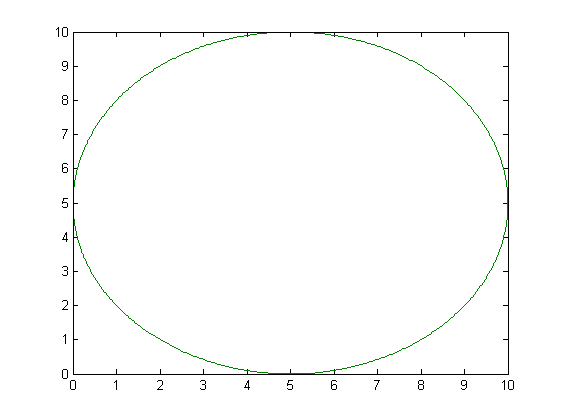
\includegraphics[width=1.0\textwidth]{testpolygon-mit_kreis.png}
\caption{Testpolygon mit Kreis}
\label{fig:testPolygon}
\end{figure}

Mit der Datei \textit{testpolygon.txt} werden die Werte $m = (472.5705, 476.6642)$ f�r den Mittelpunkt
und $r =  438.5922$ f�r den Radius des Kreises berechnet. Die entsprechende Grafik wird in der Abbildung \ref{fig:polygon} abgebildet.
Das konvexe Polygon wird blau und der gr��tm�gliche einbeschreibbare Kreis gr�n dargestellt.
\begin{figure}[htb]
\centering
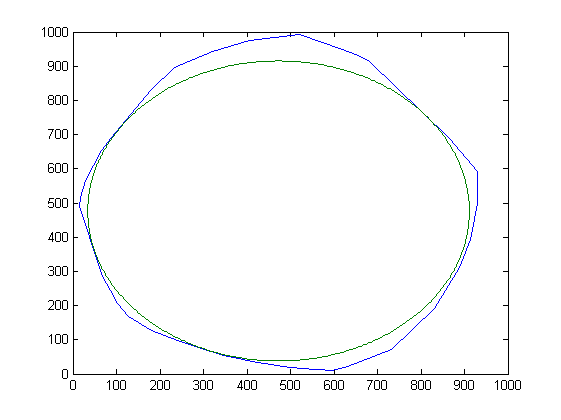
\includegraphics[width=1.0\textwidth]{polygon-mit_kreis.png}
\caption{Polygon mit Kreis}
\label{fig:polygon}
\end{figure}


\section{Aufgabe 5 - Berechnung von konvexen H�llen mit qhull}
\label{sec:Aufgabe5}
In dieser Aufgabe werden mit dem Programm \textit{qhull}\footnote{http://www.qhull.org/} zuf�llige Punktmengen erzeugt und mit diesen, eine
konvexe H�lle in verschiedenen Dimensionen berechnet.
Dabei wird zuerst ein Programm f�r die automatische Berechnung entwickelt um anschlie�end die Berechnungszeiten zu pr�sentieren.


\subsection{Programm f�r die Berechnungen}
\label{sec:programm}
Um f�r die verschiedenen Dimensionen und wechselnden Punkte die Berechnungszeiten zu ermitteln, wurde ein kleines Programm
entwickelt. Das Programm nutzt die von \textit{qhull} zur Verf�gung gestellten C++ Schnittstellen und Bibliotheken.
Die ben�tigten Bibliotheken k�nnen durch die jeweiligen Qt-Creator Projektdateien erzeugt werden.
Die Projektdatei sowie die Berechnungsergebnisse sind im Ordner \texttt{aufgabe5\\} abgespeichert.
Damit das Programm gestartet werden kann, muss es in dem \textit{qhull} Ordner \texttt{src\\} kopiert werden.
Dadurch werden alle Abh�ngigkeiten f�r das Programm verf�gbar gemacht.


\subsection{Ergebnisse der Berechnungszeiten}
\label{sec:a5ergebnisse}
In der Abbildung \ref{fig:dim2to5} werden die Berechnungszeiten f�r die Dimensionen 2 bis 5 in einem 
Koordinatensystem dargestellt. Dabei wurde eine maximale Punktemenge von $1.000.000$ zuf�llig erzeugten Punkten genutzt.
Gestartet wurde bei $0$ und schrittweise um $100.000$ Punkte bis zum Maximum erh�ht.
Die Punkte werden auf der x-Achse und die gemessenen Berechnungszeiten auf der y-Achse abgebildet.
Die Dimensionen 2 und 3 werden in der obersten und die Dimensionen 4 und 5 in der untersten Grafik gezeigt.

\begin{figure}[htb]
\centering
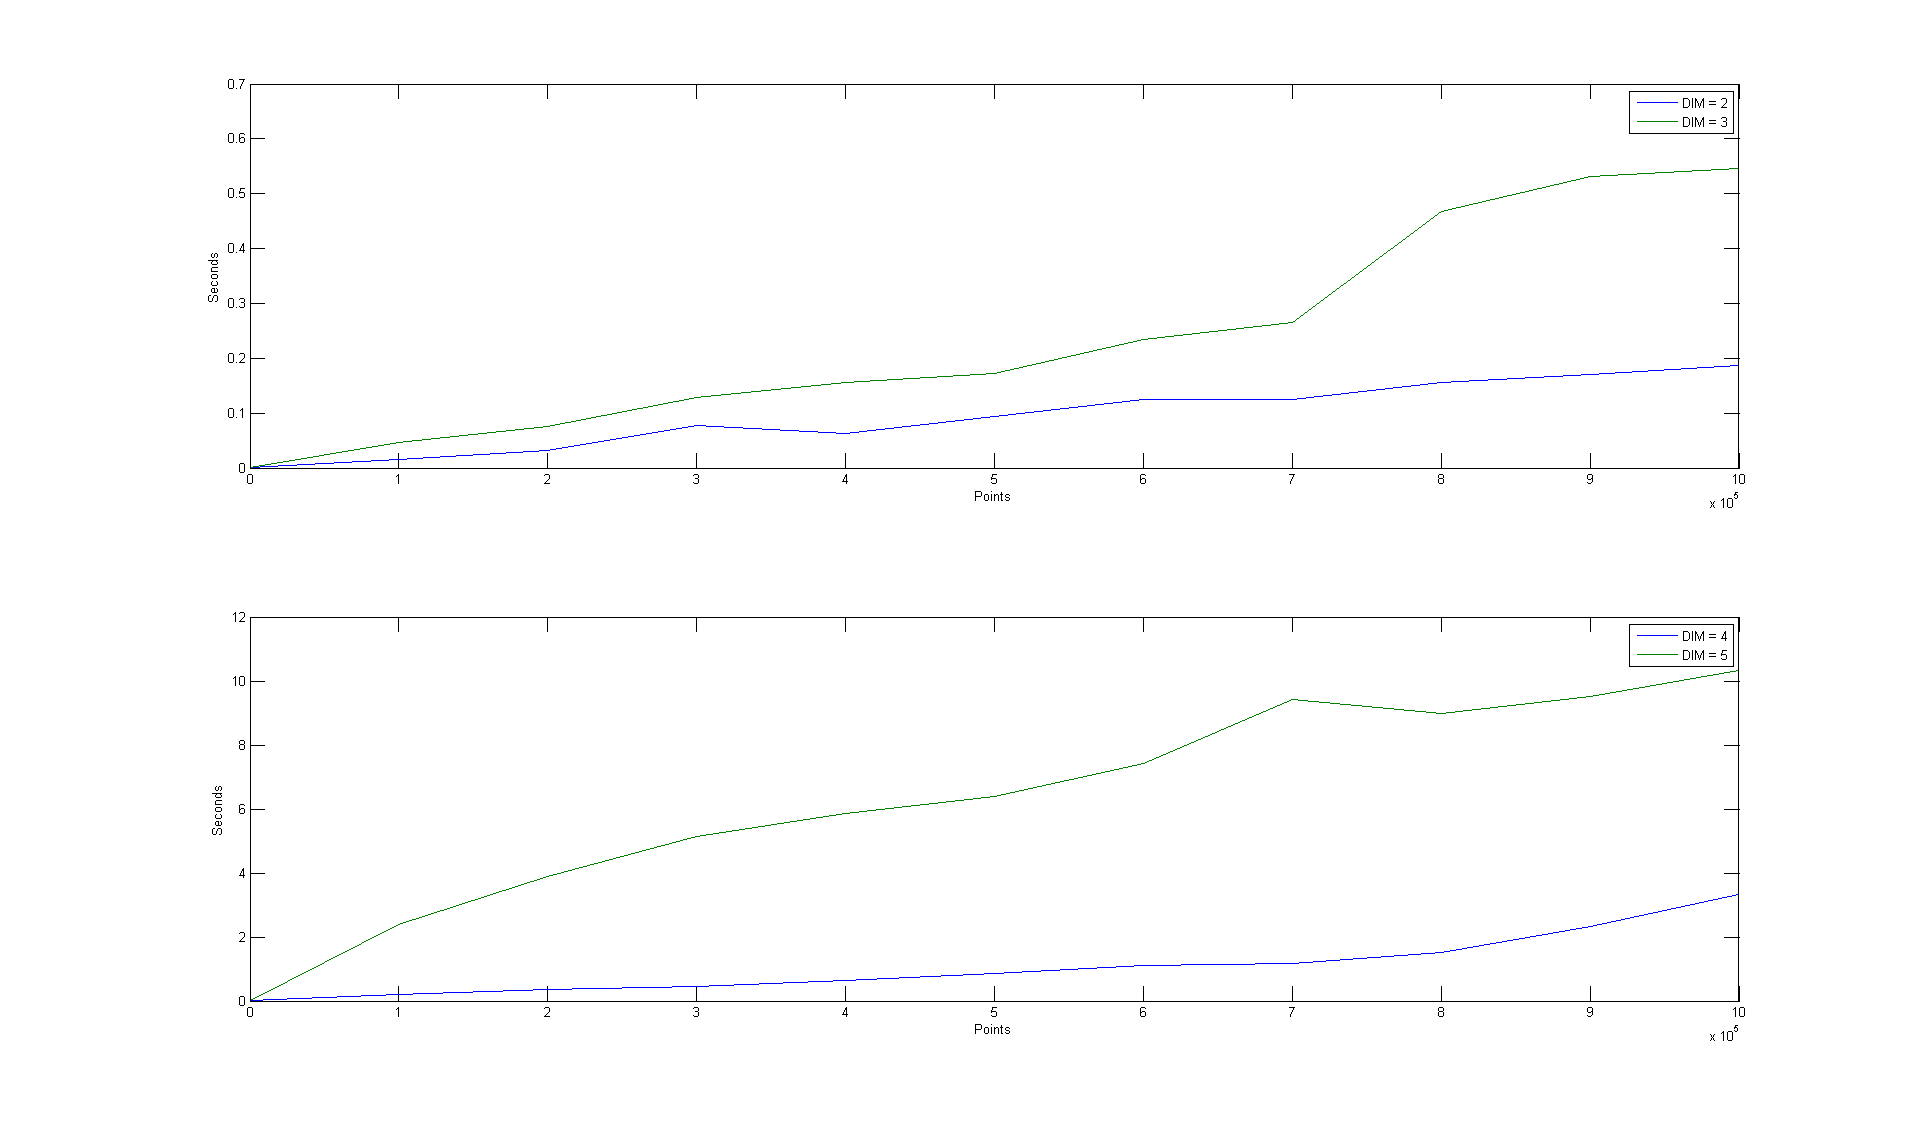
\includegraphics[width=1.0\textwidth]{dim2-5.png}
\caption{QHull Ergebnisse f�r die Dimensionen 2 - 5}
\label{fig:dim2to5}
\end{figure}

F�r die Dimensionen 6, 7 und 8 mussten die Punktemengen aufgrund von zu langen Berechnungszeiten und Arbeitsspeicher Problemen abge�ndert werden.
Die Berechnungszeiten werden in der Abbildung \ref{fig:dim6to8} in separaten Koordinatensystemen dargestellt.
Dabei wurde eine maximale Punktemenge von $1000$ Punkten mit einem Inkrementierungsschritt von $100$ Punkten verwendet. 


\begin{figure}[htb]
\centering
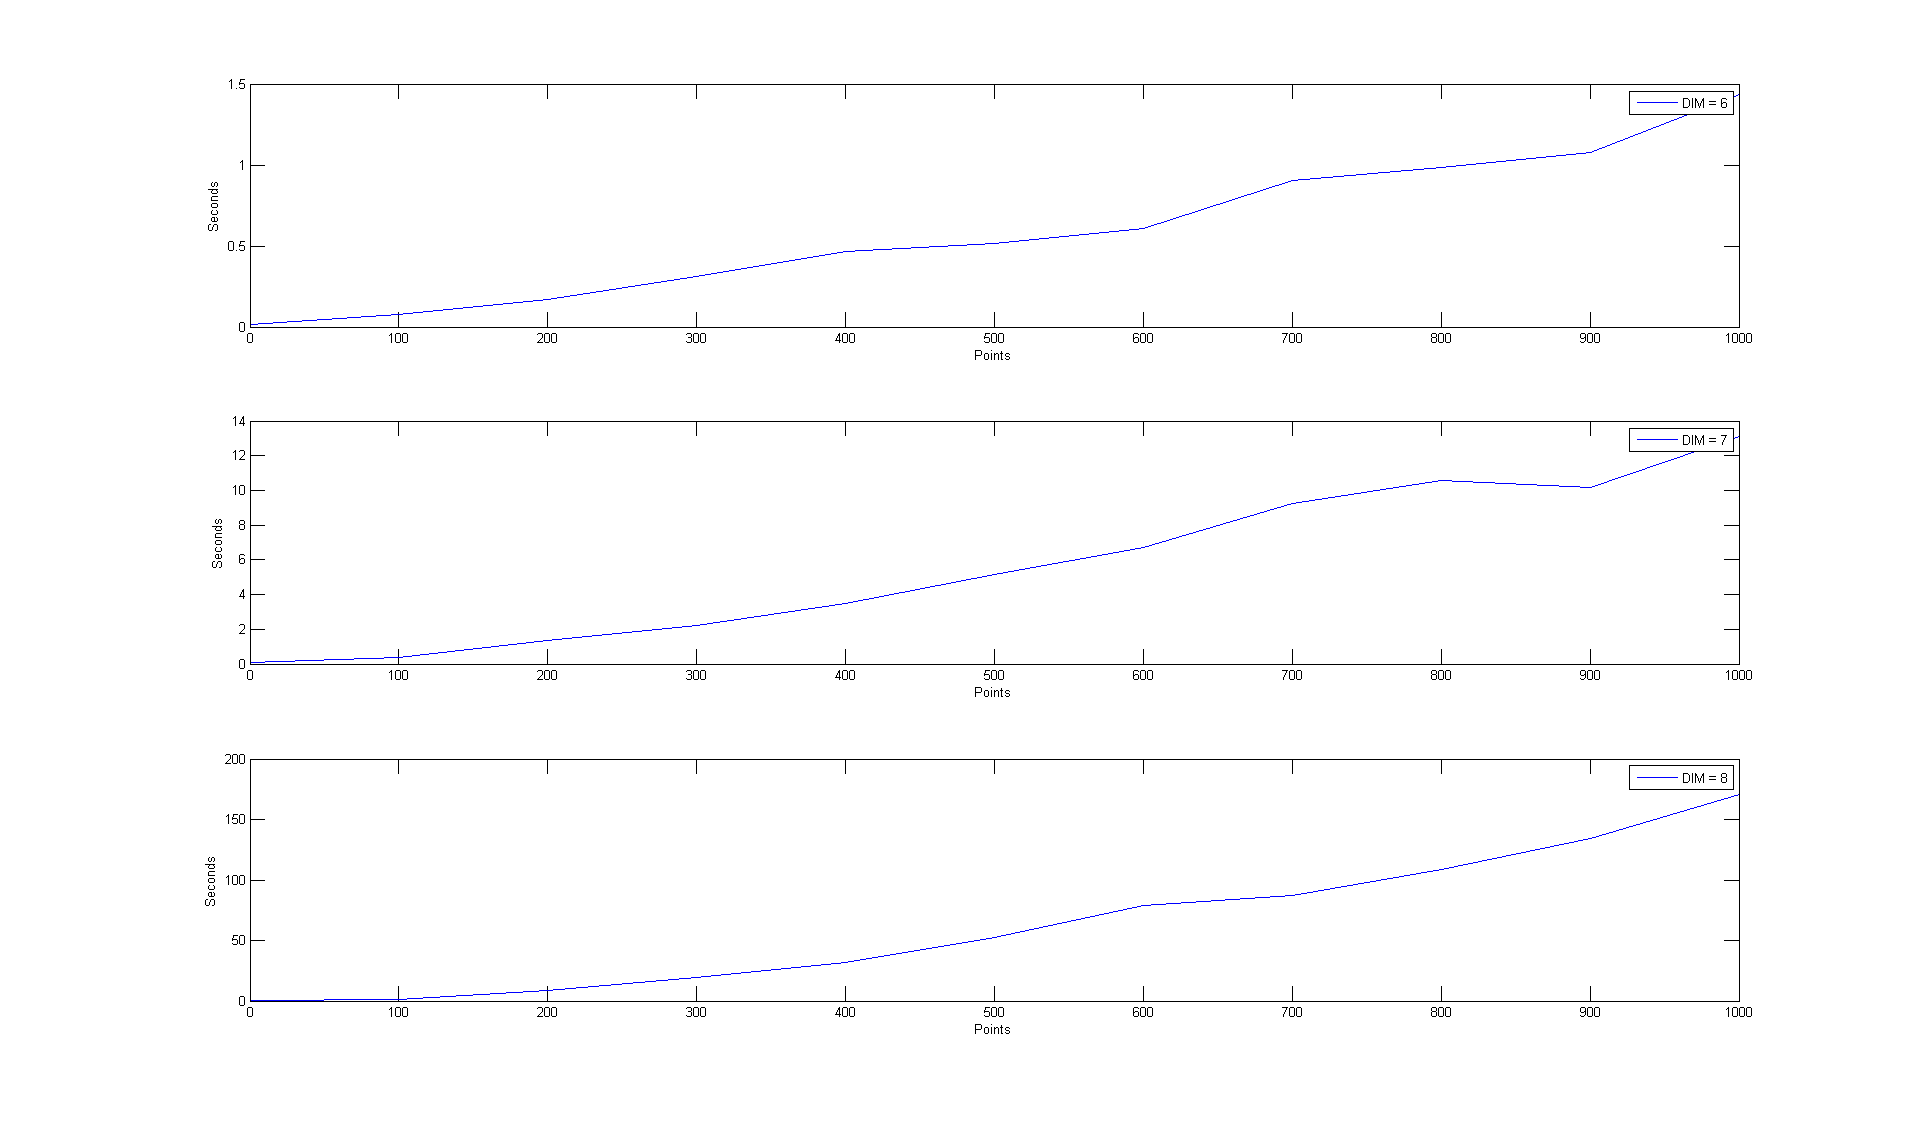
\includegraphics[width=1.0\textwidth]{dim6-8.png}
\caption{QHull Ergebnisse f�r die Dimensionen 6 - 8}
\label{fig:dim6to8}
\end{figure}
\section{Fazit}
\label{sec:Fazit}

\subsection{Zusammenfassung}
Die Aufgaben konnten alle gel�st werden, allerdings erforderten gerade die ersten drei Aufgaben sehr viel Zeit. Insgesamt musste man teilweise sehr viel Zeit f�r Dinge aufwenden, die nicht direkt mit der eigentlichen Aufgabe zu tun haben. Beispielsweise war das parsen des Input Files in der zweiten Aufgabe extrem aufwendig, wenn man nicht Java verwendet. In Aufgabe 3 war die suche nach Funktionen der STL, die man verwenden kann und die auch funktionieren wie erwartet sehr aufwendig. Die eigentliche Aufgabe war dagegen weniger komplex.

Vermutlich h�tte man sich viel Arbeit sparen k�nnen, wenn die Zusammenarbeit zwischen den Teams besser gewesen w�re. Man h�tte dann gemeinsame Parser oder gleiche STL-Funktionen verwenden k�nnen. Tats�chlich wurden allerdings nur die Ergebnisse verglichen und teilweise die Algorithmen, allerdings erst nachdem man selbst eine Implementierung konstruiert hat.

Insgesamt hat das Praktikum sehr zum Verst�ndnis und der Vertiefung des Vorlesungsstoff beigetragen. Durch die Aufgaben musste man sich mit den Problemen weiter auseinandersetzten und sich funktionierende Konzepte f�r die Realisierung �berlegen. Selbst wenn die meisten Probleme weniger mit dem Stoff, als mit der Umsetzung in Programmcode zu tun hatten, ist der R�ckblick trotzdem positiv.

\subsection{Lessons Learned}
Wir haben w�hrend des Praktikums gelernt, dass man durch Kooperation zu den besten Ergebnissen kommt. Durch die zus�tzliche Kreativit�t und Inspiration, die man durch Diskussionen mit anderen Teams bekommt, gewinnt auch die Eigene Arbeit an Qualit�t.

Aufgabe 1 hat verdeutlicht, dass es nicht einen richtigen Algorithmus gibt. Wir haben es geschafft in einem Team 2 verschiedene Realisierungen zu Implementieren. Beide Ideen haben ihre Vor- und Nachteile und da wir uns nicht einigen konnten, welcher nun besser ist haben wir uns entschieden beide unabh�ngig zu verwenden.

Sowohl die Funktion des Line Sweep, als auch die STL-Funktionen zu Listen und Vectoren wurden in Aufgabe 3 verwendet und dadruch vertieft. In dieser Aufgabe konnte man erkennen, dass lineare Laufzeiten schlechter sein k�nnen als quadratische, da man die Art der Faktoren beachten muss. Bei Outputsensiven Algorithmen muss beachtet werden ob der Input einen sinnvollen Einsatz zul�sst.






% Literaturverzeichnis ---------------------------------------------------------
%   Das Literaturverzeichnis wird aus der BibTeX-Datenbank "lit.bib"
%   erstellt.
% ------------------------------------------------------------------------------
% \nocite{*} % alles auflisten
\bibliographystyle{literatur/plaindin} % DIN-Stil des Literaturverzeichnisses
\bibliography{literatur/literatur} % Aufruf: bibtex Bachelorarbeit



% Anhang -----------------------------------------------------------------------
%   Die Inhalte des Anhangs werden analog zu den Kapiteln inkludiert.
%   Dies geschieht in der Datei "Anhang.tex".
% ------------------------------------------------------------------------------
%\begin{appendix}
%    \clearpage
%    \pagenumbering{roman}
%    \chapter{Anhang}
%    \label{sec:Anhang}
%     Rand der Aufz?hlungen in Tabellen anpassen
%    \setdefaultleftmargin{1em}{}{}{}{}{}
%    \section{Quellcode}


%\end{appendix}

% Index ------------------------------------------------------------------------
%   Zum Erstellen eines Index, die folgende Zeile auskommentieren.
% ------------------------------------------------------------------------------
%\printindex

\end{document}
